% !TeX spellcheck = cs_CZ
{\tikzset{external/prefix={tikz/FYZI/}}
 \tikzset{external/figure name/.add={ch52_}{}}
%=========================== Kapitola: Symetrie fyzikálních zákonů ================================
\chapter{Symetrie fyzikálních zákonů}\label{fyz:IchapLII}
\minitoc
  \section{Symetrické operace}\label{fyz:IchapLIIsecI}
  \section{Symetrie v prostoru a čse}\label{fyz:IchapLIIsecII}
  \section{Symetrie a zákony zachování}\label{fyz:IchapLIIsecIII}
  \section{Zrcadlový obraz}\label{fyz:IchapLIIsecIV}
  \section{Polární a axiální vektory}\label{fyz:IchapLIIsecV}
  \section{Parita se nezachovává}\label{fyz:IchapLIIsecVI}
  \section{Antihmota}\label{fyz:IchapLIIsecVII}
  \section{Porušení symetrie}\label{fyz:IchapLIIsecVIII}
  \section{Příklady a cvičení}\label{fyz:IchapLIIsecIX}
  
    \begin{figure}[ht!] %\ref{fyz_fig441}
      \centering
      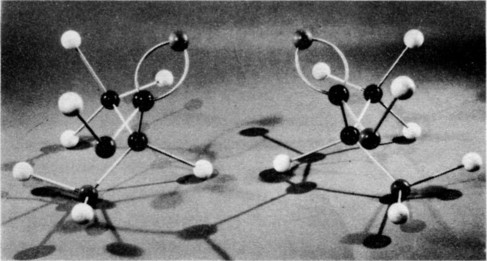
\includegraphics[width=0.7\linewidth]{fyz_fig441.jpg}
      \caption{
               (\cite[s.~704]{Feynman01})}
      \label{fyz_fig441}
    \end{figure}

    \begin{figure}[ht!] %\ref{fyz_fig442}
      \centering
      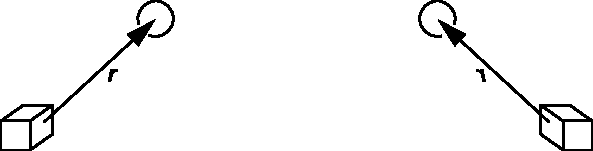
\includegraphics[width=0.7\linewidth]{fyz_fig442.pdf}
      \caption{Posunutí v prostoru a jeho zrcadlový obraz
               (\cite[s.~706]{Feynman01})}
      \label{fyz_fig442}
    \end{figure}

    \begin{figure}[ht!] %\ref{fyz_fig443}
      \centering
      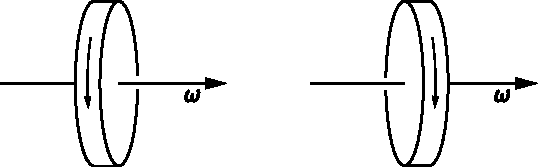
\includegraphics[width=0.7\linewidth]{fyz_fig443.pdf}
      \caption{Rotující kolo a jeho zrcadlový obraz. Všimněme si že směr \uv{vektoru} úhlové 
               rychlosti se nezměnil 
               (\cite[s.~706]{Feynman01})}
      \label{fyz_fig443}
    \end{figure}

    \begin{figure}[ht!] %\ref{fyz_fig444}
      \centering
      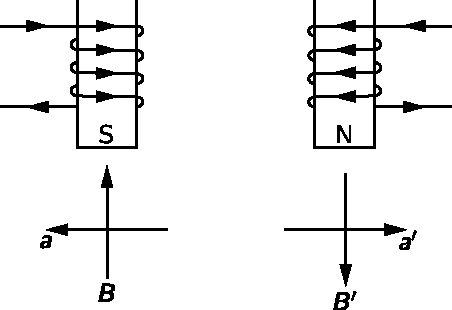
\includegraphics[width=0.7\linewidth]{fyz_fig444.pdf}
      \caption{Magnet a jeho zrcadlový obraz 
               (\cite[s.~707]{Feynman01})}
      \label{fyz_fig444}
    \end{figure}
    
    \begin{figure}[ht!]      %\ref{fyz:fig445}
      \centering
      \begin{tabular}{cc}
        \subfloat[ ]{\label{fyz:fig445a}
          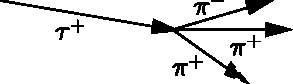
\includegraphics[width=0.4\linewidth]{fyz_fig445a.pdf}}
        \hspace{-1em}                                                       &
        \subfloat[ ]{\label{fyz:fig445b}
          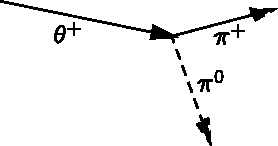
\includegraphics[width=0.4\linewidth]{fyz_fig445b.pdf}}
      \end{tabular}
      \caption{Schématický diagram rozpadu \(\tau^+\) a \(\Theta^+\)
               \cite[s.~708]{Feynman01}}
      \label{fyz:fig445}
    \end{figure}


} %tikzset
%---------------------------------------------------------------------------------------------------
\printbibliography[title={Seznam literatury}, heading=subbibliography]
\addcontentsline{toc}{section}{Seznam literatury}